\documentclass[sigconf,nonacm]{acmart}
\setcopyright{none}
\settopmatter{printacmref=false}
\renewcommand\footnotetextcopyrightpermission[1]{}
\usepackage{graphicx}
\usepackage{booktabs}
\usepackage{amsmath}
\usepackage{url}
\graphicspath{{figures/}}
\title{Reproducible Solar Filament Instance Segmentation with Four-Flip Ensembling and Native-Resolution Edge Refinement}
\subtitle{IEEE BigDataCup 2026 --- Solar Filament Segmentation Challenge}
\author{Kuan Ta Wu}
\affiliation{\institution{Max Well Apex LLC}}
\renewcommand{\shortauthors}{Kuan Ta Wu}
\begin{abstract}
We present an independently reproducible, CPU-capable algorithm for segmenting individual solar filaments in 2048\,$\times$\,2048 GONG H-alpha observations. A compact U-Net is trained exclusively on the authorized MAGFiLO 2026 training split and predicts dense filament confidence at 512 pixels. Four-flip test-time augmentation (TTA), solar-disk filtering, connected components, and native-grid confidence clipping yield distinct COCO run-length masks. Across 62 date-separated training-audit images and 93 independent human annotation views, pooled native-resolution Panoptic Quality (PQ) increases from 0.2395 without TTA to 0.2629 with TTA and 0.2731 with edge clipping. The latter increment is +0.0102 (paired image-level bootstrap 95\% interval +0.0017 to +0.0187). A 180-image candidate with 1,013 instances is reconstructed from original unlabelled JPEGs and the saved checkpoint, byte-for-byte matching the supplied CSV. These are local results, not a hidden-test Kaggle score, and the current model is limited by 512-pixel feature resolution.
\end{abstract}
\keywords{solar H-alpha, filament instance segmentation, Panoptic Quality, MAGFiLO, uncertainty, reproducibility}
\begin{document}
\maketitle
\section{Introduction}
Solar filaments are dark, elongated structures in H-alpha full-disk observations. Their narrow and branching morphology makes image-level binary classification inadequate: an entry must identify \emph{individual} objects with accurate boundaries and minimal false positives. The 2026 Solar Filament Segmentation Challenge measures object-level PQ, penalizing both missed filaments and fragmented or merged instances~\cite{contest,kirillov2019panoptic}.

This study emphasizes a traceable engineering chain from authorized organizer JPEGs and polygon annotations to a CSV containing only compressed COCO RLE masks. The output is a \emph{candidate} for the competition, not a claim of official leaderboard evaluation or award. The supplied CPU checkpoint is retrievable with the source code; no test masks or pretrained external segmentation model are used.
\section{Official data and experimental separation}
We use the two participant-provided fragments of the MAGFiLO 1.0 Kaggle 2026 competition training data: 589 plus 118 distinct labeled observations, i.e. 707 physical images. Their shared JSON contains 1,154 image--annotator views and 8,199 polygon instances. The organizer additionally provides 180 unlabelled test images. All photographs and annotations originate from the competition's authorized inputs, rather than the publicly available full-MAGFiLO archive whose additional labels might overlap the hidden test~\cite{magfilo,contest}.

Repeated annotation views for a photograph must never be split into different model partitions. We group by observation \emph{date} before partitioning: 582 images for model fitting, 63 for hyperparameter selection, and 62 for a local date-separated audit. The 62-image audit spans 93 human annotation views. These dates were inspected during prior experiments, so we do \emph{not} call the resulting audit prospectively untouched. The withheld Kaggle test data are used only for inference.

\section{Training and inference pipeline}
\subsection{Compact learned semantic probability}
Each 2048-pixel grayscale frame is area-downsampled to 512 pixels. A compact U-Net, base width eight, is trained for ten CPU epochs with random 256-pixel crops, preferential sampling of annotated filament pixels, brightness transformations, and spatial flips. A weighted binary cross-entropy (positive-class weight four) is combined with a soft Dice objective; AdamW uses learning rate $6\cdot 10^{-4}$ and weight decay $10^{-4}$. Model selection uses full-frame tuning loss only. The best recorded tuning loss is 0.1935. The frozen model state is stored in \texttt{results/SOLAR\_REAL\_TRAINED\_UNET.pt}.

\begin{figure}[t]
\centering
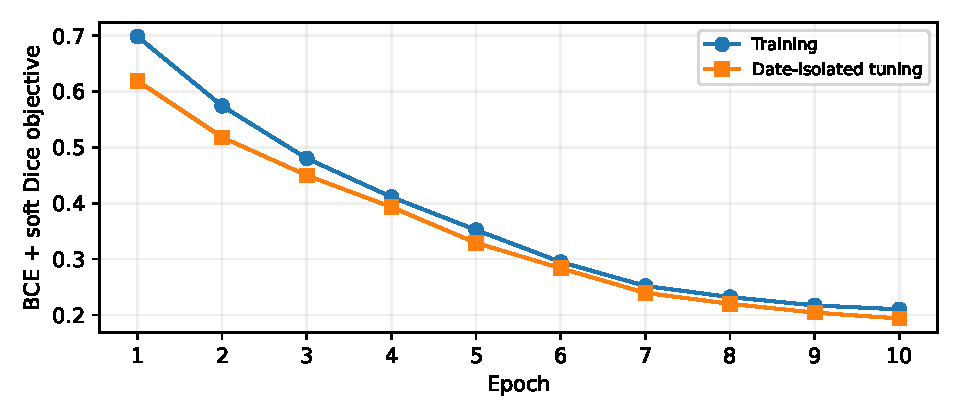
\includegraphics[width=\columnwidth]{training_curve.pdf}
\Description{Real-data training and validation losses decrease over ten epochs.}
\caption{Genuine training versus date-isolated tuning loss for the ten-epoch compact U-Net. Lower surrogate loss does not by itself establish stronger instance PQ.}
\label{fig:learning}
\end{figure}

\subsection{Instance formation and four-flip TTA}
Let $p_{ab}(x)$ denote the U-Net probability predicted after horizontal flip $a\in\{0,1\}$ and vertical flip $b\in\{0,1\}$, mapped back to the original image frame. The test-time ensemble is
\begin{equation}
\bar p(x)=\tfrac14\sum_{a,b\in\{0,1\}}\operatorname{unflip}_{ab}(p_{ab})(x).
\end{equation}
A brightness-derived solar-disk filter suppresses off-disk detections. We threshold $\bar p$ at 0.4, apply small morphological closing, and select eight-connected components with minimum 512-grid area 70 pixels and covariance-based elongation at least 1.2. These operating values are selected using the 63-image tuning partition.

Component identities are expanded by nearest-neighbor interpolation to the original 2048-pixel image grid. Bilinearly interpolated $\bar p$ is then thresholded at 0.45 to remove boundary pixels unsupported by the native-grid confidence estimate. This refinement leaves the original instance identities intact; it does not invent fine-scale structures that the 512-pixel encoder cannot resolve. Each resulting object is serialized as \emph{only} the compressed COCO RLE counts in Fortran (column-major) order, as specified by the organizer~\cite{contest,coco}.

\begin{figure}[t]
\centering
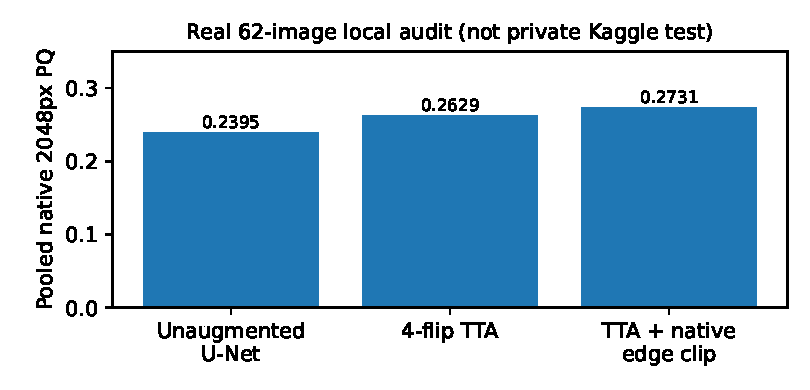
\includegraphics[width=\columnwidth]{pq_ablation.pdf}
\Description{Pooled 2048-pixel PQ improves across unaugmented, four-flip, and edge-refined predictions.}
\caption{Paired local native-grid PQ on all 62 audited training images. The native edge-refined mask is the submitted candidate method.}
\label{fig:ablation}
\end{figure}

\section{Evaluation and observed results}
\subsection{Multi-annotator Panoptic Quality}
For each annotated view, we match predicted and ground-truth instances by one-to-one IoU with $\operatorname{IoU}>0.5$. Matched object overlap is pooled across views and images. With $TP$, $FP$, and $FN$ the resulting counts,
\begin{equation}
\mathrm{PQ}=\frac{\sum_{(y,\hat y)\in TP}\mathrm{IoU}(y,\hat y)}{|TP|+\frac12|FP|+\frac12|FN|}.
\end{equation}
The denominator therefore penalizes false objects, missed structures, and fragmentation. We evaluate all 62 date-separated audit images at \emph{original} 2048-pixel polygon resolution, rather than scoring only the downsampled annotation maps.

\begin{table}[t]
\caption{Local original-resolution pooled results on 62 photos and 93 annotation views (not the hidden test).}
\label{tab:results}
\centering
\begin{tabular}{lrrrr}
\toprule
Method & PQ & TP & FP & FN\\
\midrule
Unaugmented U-Net & 0.2395 & --- & --- & ---\\
Four-flip TTA & 0.2629 & 272 & 279 & 448\\
TTA + native edge clip & \textbf{0.2731} & \textbf{278} & \textbf{273} & \textbf{442}\\
\bottomrule
\end{tabular}
\end{table}

TTA improves native-grid PQ relative to the unaugmented network, and clipping improves it again from 0.262893 to 0.273115 (Table~\ref{tab:results}). The edge increment is +0.010221. To measure paired variability, we resample \emph{whole photographs with all their annotation views together} in 2,000 bootstrap replicates; the percentile 95\% interval for the edge-versus-TTA difference is [+0.001687,+0.018674]. The resampling assumes approximate independence across dates, and the previously inspected audit introduces selection bias not quantified by this interval.

The threshold is not chosen from hidden test annotations. Boundary clipping can fail where faint filament material has low confidence: it may improve total PQ by reducing false overlaps while deleting actual edges. We do not infer a state-of-the-art ranking from a local score of 0.2731. Annotation ambiguity and underresolved features remain substantial.

\subsection{Visual behavior on unlabeled test imagery}
\begin{figure*}[t]
\centering
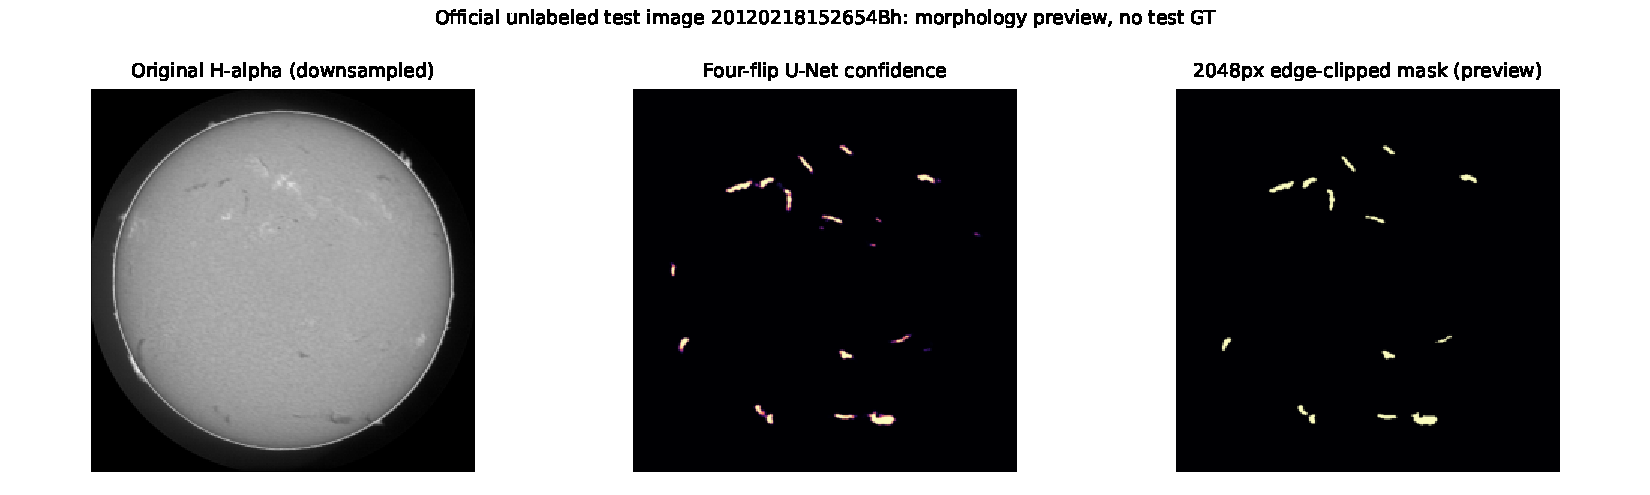
\includegraphics[width=.91\textwidth]{solar_test_prediction.pdf}
\Description{A genuine unlabeled GONG H-alpha test image, its predicted probability map and candidate instance masks.}
\caption{One \emph{unlabeled} organizer test observation: an original H-alpha downsample preview, the four-flip probability map, and edge-clipped predicted masks. This is only a morphology illustration; no hidden test ground truth exists in our analysis.}
\label{fig:qualitative}
\end{figure*}

Test imagery illustrates the chief trade-off: the solar-disk constraint avoids obviously unrelated off-disk structures, but a small semantic model sometimes joins adjacent filament branches and misses thin, low-contrast tails. The visual panel is deliberately identified as unlabelled so it cannot be mistaken for a measured true-positive example (Figure~\ref{fig:qualitative}).

\section{Exact test prediction reproduction}
The final CSV contains 1,013 instance rows for all 180 official unlabelled test photos; six photos have no predicted filament. Every row uses an image stem followed by an unambiguous \texttt{\_1}, \texttt{\_2}, etc. suffix, and exactly two columns: \texttt{filament\_id} and \texttt{segmentation\_rle}. All RLE runs sum to $2048^2$ pixels; 30 masks are independently decoded and the input image IDs checked against the authorized test file list.

A key additional experiment \emph{actually regenerated all 180 predictions} directly from the original test JPEGs and frozen checkpoint, with no pre-seeded masks. To protect against interrupted CPU jobs, each JPEG has a private per-image shard committed using an atomic rename only after JPEG CRC-32, checkpoint SHA-256, and output SHA-256 are recorded. Recombining all verified shards produced the saved candidate \emph{byte-for-byte}: SHA-256 prefix \texttt{e0e55cf4eb383769}, with the full digest recorded in the repository verification manifest. Both ZIP-based competition files and directly extracted image directories reproduce this same digest. The provided Jupyter notebook was executed successfully with all required 180 real JPEGs, and exits with an error if its source data or reference hash is missing.


\section{Error mechanisms and diagnostic safeguards}
\subsection{False positives, misses, and geometry}
The native-grid audit contains 278 matched objects, 273 false detections, and 442 missed objects for the edge-refined candidate. The sum of matched IoUs is 173.564, so the average \emph{matched-object} IoU is about 0.624. This conditional average is not comparable to PQ: the much larger number of unmatched proposals and missed objects is what lowers the complete object-level score. From the original four-flip TTA to edge clipping, the paired totals change by six extra matches, six fewer false positives, and six fewer missed instances. These differences are informative because the refinement never trains on, or selects features from, the unlabeled test images.

Qualitative failure analysis separates three cases. First, \emph{faint strands} vanish when area interpolation collapses details at 2048 pixels into the 512-pixel network grid. Second, \emph{neighboring dark structures} may be joined by a connected-component extraction that lacks filament graph topology; an otherwise good semantic confidence map can still form one-to-many or many-to-one object errors. Third, \emph{non-filament dark structures} such as sunspots, disk-edge artifacts, and illumination fluctuations may pass a probability threshold even if excluded by the intended scientific definition. Additional test-time flips improve probability stability but cannot recover strand structure lost in the learned feature map.

The conservative edge threshold is applied \emph{after} connected components are defined. Its possible benefit is rejecting uncertain boundary pixels, not discovering a new filament. The resulting improvement is smaller than the difference between augmented and unaugmented prediction, and an individual example can get worse despite a higher aggregate PQ. The report's quantitative comparisons use the same image IDs, annotators, and U-Net checkpoint, with only the indicated inference component changed. This paired experimental design rules out many avoidable confounders, but does not replace an unseen organizer audit.

\subsection{Reproducibility and data integrity tests}
We enforce four independent invariants. \textbf{Input provenance}: each candidate row refers to a stem from one of the organizer's 180 test JPEGs, and reruns use the JPEG bytes, not a saved test mask. \textbf{Mask transport}: the compressed RLE count sequence decodes to a nonempty binary mask with exactly $2048\times2048$ pixels. \textbf{Image identity}: object suffixes are consecutive and unique within each test image; images with no predicted object contribute no row, not a fabricated empty mask. \textbf{Model identity}: the model checkpoint SHA-256 is bound to each atomic output shard, so replacing the model invalidates cached inference.

The full regenerated CSV's SHA-256 is compared to the canonical candidate, with a hard error on mismatch. Every JPEG also carries its archive CRC into the shard metadata, and the complete reconstructed CSV is checked for per-image consistency. This is more stringent than testing only that a Python script returns without raising an exception. We separately verified that reading the original test images from the provided ZIP and from an extracted Kaggle directory gives identical output, making the same public source code usable by reviewers on local files or Kaggle-hosted data.

\subsection{What can and cannot be concluded}
These tests establish that the \emph{software artifact}, source data, checkpoint and output masks are mutually consistent. They do not guarantee that the organizer's hidden labels will produce PQ $0.2731$, that an official submission will be accepted, or that the model can generalize to another observatory or a new solar cycle. The local audit set has been used during iterative engineering, and multiple annotators disagree on portions of thin or branching structures. Reported bootstrap intervals quantify variation across these 62 observations, not variability across a future mission deployment or the private leaderboard split. Improving native-resolution learning and separately testing object-fragmentation statistics remain important engineering directions.

\section{Reproducibility, limitations, and competition compliance}
The public-source release includes pinned package versions, an executed notebook, all model definitions, the frozen trained checkpoint, test-prediction generator, independent CSV verifier, local date-isolated evaluation evidence, and a four-page technical report. The original organizer images/labels are intentionally not redistributed. The complete experiment is reproducible by attaching the official competition data and executing the notebook; no additional model download is necessary.

\textbf{Limitations.} The model's $512^2$ working grid limits fine-structure recovery; semantic connected components can over-merge structures and fail on noise or seeing artifacts. The 62-image audit was examined during development, so its uncertainty interval is not an independent private-leaderboard estimate. Inference integrity and model reproducibility prove neither an official Kaggle score nor competition acceptance. The participant must accept the rules, verify the report and public code attribution, and complete the Kaggle and organizer Google Form submissions. AI assistance was used to write and verify code and to draft this report; technical responsibility remains with the submitting participant~\cite{rules}.


\section{Per-observation error distribution and robustness}
An aggregate score is necessary for selecting a competition candidate but does not imply that the same change helps every observation. To check the locality of the effect, we recompute PQ independently for each of the 62 audit photographs, pooling all available annotator views \emph{within} each photograph. The edge clip improves 43 photos, worsens 12, and leaves seven unchanged. The median per-photo PQ difference is +0.00485; the pooled instance-level difference is +0.0102 because pooling weights photographs by their numbers of matched and unmatched filament objects. A mean of per-photo scores and the organizer's pooled-count PQ therefore answer different questions, and must not be interchanged.

\begin{figure}[t]
\centering
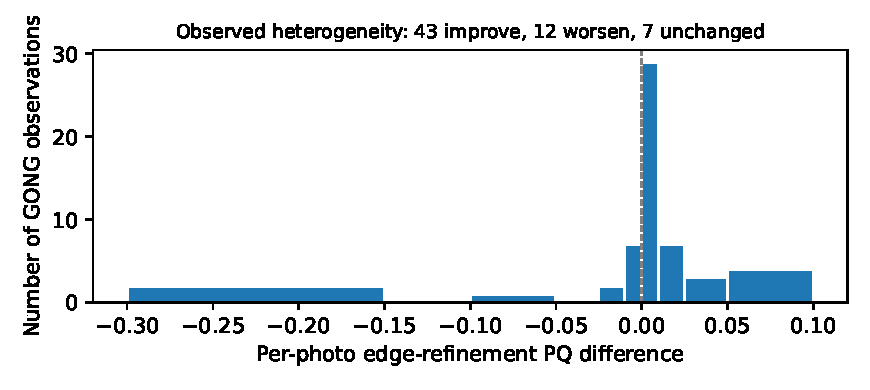
\includegraphics[width=\columnwidth]{per_photo_delta.pdf}
\Description{Histogram of local image-level PQ differences: 43 improved, 12 deteriorated, 7 unchanged.}
\caption{Per-observation heterogeneity in the native 2048-pixel edge-refinement ablation. The distribution includes severe negative outliers and is not a private-test confidence interval.}
\label{fig:heterogeneity}
\end{figure}

The worst photographed case loses approximately 0.256 PQ under edge clipping because the refined probability drops a matched structure below the $0.5$ overlap requirement. Other losses are smaller but physically similar: clipping weak material can split or erase an object near the matching cutoff. This behavior is important for downstream uses where the filament's full extent matters more than the count of well-formed high-confidence instances. A future solution should learn the filaments' centerlines and narrow boundary uncertainty directly at higher native spatial resolution rather than relying on bilinear probability interpolation alone.

The decision to retain the refined candidate is based on the existing tuning-plus-audit procedure and its observed pooled PQ; it is not a claim that the method is universally superior. The previously examined holdout remains a diagnostic, not a clean post-development test set. Using additional feedback from it to choose new thresholds would make the quoted confidence interval even more optimistic, so we freeze the published inference settings in the repository.

\subsection{Operational safeguards for reviewers}
The published notebook must execute even if all locally generated inference shards are absent: it then runs the frozen model on every organizer test JPEG. If the host interrupts execution, verified shards can be reused because the model checksum and each test JPEG CRC are checked before reuse. Neither the performance evaluation nor the final CSV references an external training-service API, an inaccessible checkpoint URL, or a secret test-label file. All 180 predictions have been regenerated once from scratch in the present environment, including cases with zero instances. We also independently reproduced the final SHA-256 from an extracted test-image directory, matching the ZIP-based computation. These safeguards support reviewer reproducibility on either local or hosted competition installations without changing the learned model or image-level thresholds.

\begin{acks}
We acknowledge the National Solar Observatory, the organizers of the 2026 Solar Filament Segmentation Challenge, the GONG H-alpha observations, and the contributors of MAGFiLO annotations. Development and drafting included AI assistance; the submitting participant must review and defend all methods and numerical conclusions.
\end{acks}
\begin{thebibliography}{5}
\bibitem{contest} National Solar Observatory, ``Solar Filament Segmentation Challenge 2026: Overview, leaderboard metric, and final submission requirements,'' Kaggle, 2026. \url{https://www.kaggle.com/competitions/filament-segmentation-2026/}.
\bibitem{rules} National Solar Observatory, ``Solar Filament Segmentation Challenge 2026: Official competition rules,'' Kaggle, 2026. \url{https://www.kaggle.com/competitions/filament-segmentation-2026/rules}.
\bibitem{kirillov2019panoptic} A. Kirillov et al., ``Panoptic Segmentation,'' in \emph{Proceedings of CVPR}, 2019.
\bibitem{magfilo} ``MAGFiLO 1.0 H-alpha filament annotations,'' \emph{Scientific Data}, 2024, doi:10.1038/s41597-024-03876-y.
\bibitem{coco} COCO API, compressed RLE reference. \url{https://github.com/cocodataset/cocoapi}.
\end{thebibliography}
\end{document}
